\documentclass[a4paper,11pt]{article}
\usepackage[margin=2.2cm]{geometry}
\usepackage{graphicx}
\usepackage{hyperref}
\usepackage{xcolor}
\usepackage{enumitem}
\usepackage{tikz}
\usetikzlibrary{arrows.meta,positioning,shapes.geometric}
\hypersetup{colorlinks=true,linkcolor=blue!60!black,urlcolor=blue!60!black}
\setlist[itemize]{topsep=2pt,itemsep=2pt}

\title{Arithmos Calculator --- DevOps Pipeline Mini-Project Report}
\author{Kaushalraj Puwar}
\date{October 2026}

\begin{document}
\maketitle

\section{Overview}
Arithmos is a small but production-style Calculator REST API in Java 21
(Spring Boot, Maven-built executable JAR), wrapped in a fully automated
DevOps pipeline using only the pre-midterm toolchain: Git/GitHub for
version control, Jenkins for CI/CD, Docker for containerization, and
Docker Compose for deployment. A push to \texttt{main} triggers a
pipeline that builds, tests, packages, containerizes, pushes, and
deploys with no manual steps.

Links: GitHub repository
\url{https://github.com/KaushalrajPuwar/arithmos-pipeline} \quad
Docker Hub image
\url{https://hub.docker.com/r/kaushalrajpuwar/arithmos-calculator}

\section{Application}
Four endpoints under \texttt{/api/v1} (\texttt{add}, \texttt{subtract},
\texttt{multiply}, \texttt{divide}) accept numeric \texttt{a}, \texttt{b}
query parameters and return
\texttt{\{"operation","a","b","result"\}} as JSON. Division by zero and
invalid or missing parameters return HTTP~400 with a structured error
body (\texttt{timestamp}, \texttt{status}, \texttt{error},
\texttt{message}, \texttt{path}) produced by a global exception handler.
Spring Actuator exposes \texttt{/actuator/health} (UP/DOWN), which the
container runtime uses as the Compose health check.

\section{Testing}
JUnit~5 service tests cover every operation including the
divide-by-zero case (now 8 tests after a decimal-addition case was added
as the live-demo change), plus 7 Spring MockMvc web-slice tests that hit
real endpoints and assert the JSON contract and both 400 error paths.
All 15 tests run via \texttt{mvn test} and emit JUnit XML under
\texttt{target/surefire-reports/}, which Jenkins publishes with the
\texttt{junit} step and fails the build on any failure.

\section{Pipeline architecture}
\begin{center}
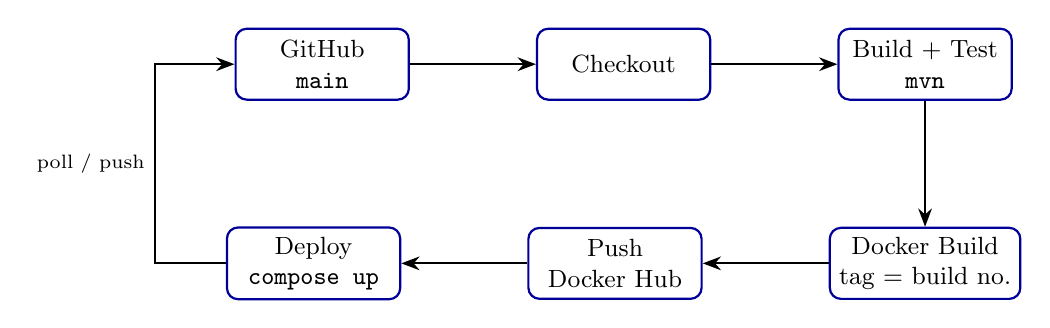
\begin{tikzpicture}[node distance=1.6cm,>=Stealth,
  box/.style={rectangle,rounded corners,draw=blue!60!black,thick,minimum width=2.2cm,minimum height=0.9cm,align=center,font=\small},
  arrow/.style={->,thick}]
  \node[box] (git) {GitHub\\\texttt{main}};
  \node[box,right=of git] (ck) {Checkout};
  \node[box,right=of ck] (bt) {Build + Test\\\texttt{mvn}};
  \node[box,below=of bt] (dk) {Docker Build\\tag = build no.};
  \node[box,left=of dk] (push) {Push\\Docker Hub};
  \node[box,left=of push] (dep) {Deploy\\\texttt{compose up}};
  \draw[arrow] (git) -- (ck);
  \draw[arrow] (ck) -- (bt);
  \draw[arrow] (bt) -- (dk);
  \draw[arrow] (dk) -- (push);
  \draw[arrow] (push) -- (dep);
  \draw[arrow] (dep.west) -- ++(-0.9,0) |- (git.west) node[pos=0.25,left,font=\scriptsize]{poll / push};
\end{tikzpicture}
\end{center}

The declarative \texttt{Jenkinsfile} defines six stages. \textbf{Checkout}
pulls the latest \texttt{main}. \textbf{Build} runs
\texttt{mvn clean package -DskipTests} pinned to Homebrew Java~21.
\textbf{Test} runs \texttt{mvn test} and archives JUnit XML.
\textbf{Docker Build} builds the multi-stage image tagged with both the
Jenkins build number and \texttt{latest}. \textbf{Push} logs in with the
Jenkins-managed \texttt{dockerhub-creds} credential (never hard-coded)
and pushes both tags. \textbf{Deploy} runs
\texttt{docker compose down --remove-orphans} then
\texttt{docker compose up -d} (idempotent re-runs), waits for
\texttt{/actuator/health} to report UP, then verifies an end-to-end call
through the Nginx proxy. Triggers are \texttt{githubPush()} with
\texttt{pollSCM('H/2 * * * *')} as fallback, and every build sends a
success/failure email via Gmail SMTP. Build~\#6 proved the loop: a test
commit pushed from a laptop was picked up automatically and deployed.

\section{Docker and Compose}
The multi-stage \texttt{Dockerfile} compiles in a Maven/JDK~21 stage
(dependencies copied first for layer caching) and copies only the JAR
into a slim JRE Alpine runtime that runs as non-root user
\texttt{app} with an explicit \texttt{EXPOSE 8080}. A single
\texttt{docker run -p 8080:8080} serves the API.
\texttt{docker-compose.yml} orchestrates two containers on one network:
\texttt{calculator} (host 8081, restart policy, Actuator health check,
\texttt{APP\_PORT} env support) and an Nginx reverse proxy (host 8082)
that only starts once the calculator is \texttt{healthy}. One
\texttt{docker compose up -d} launches the full stack.

\section{Evidence}
Build~\#5 (and later auto-triggered build~\#6) ran fully green: all six
stages plus JUnit archiving and the success email. The deployed stack
answers through both the proxy (\texttt{:8082}) and the app directly
(\texttt{:8081}), with divide-by-zero correctly returning HTTP~400.

\begin{center}
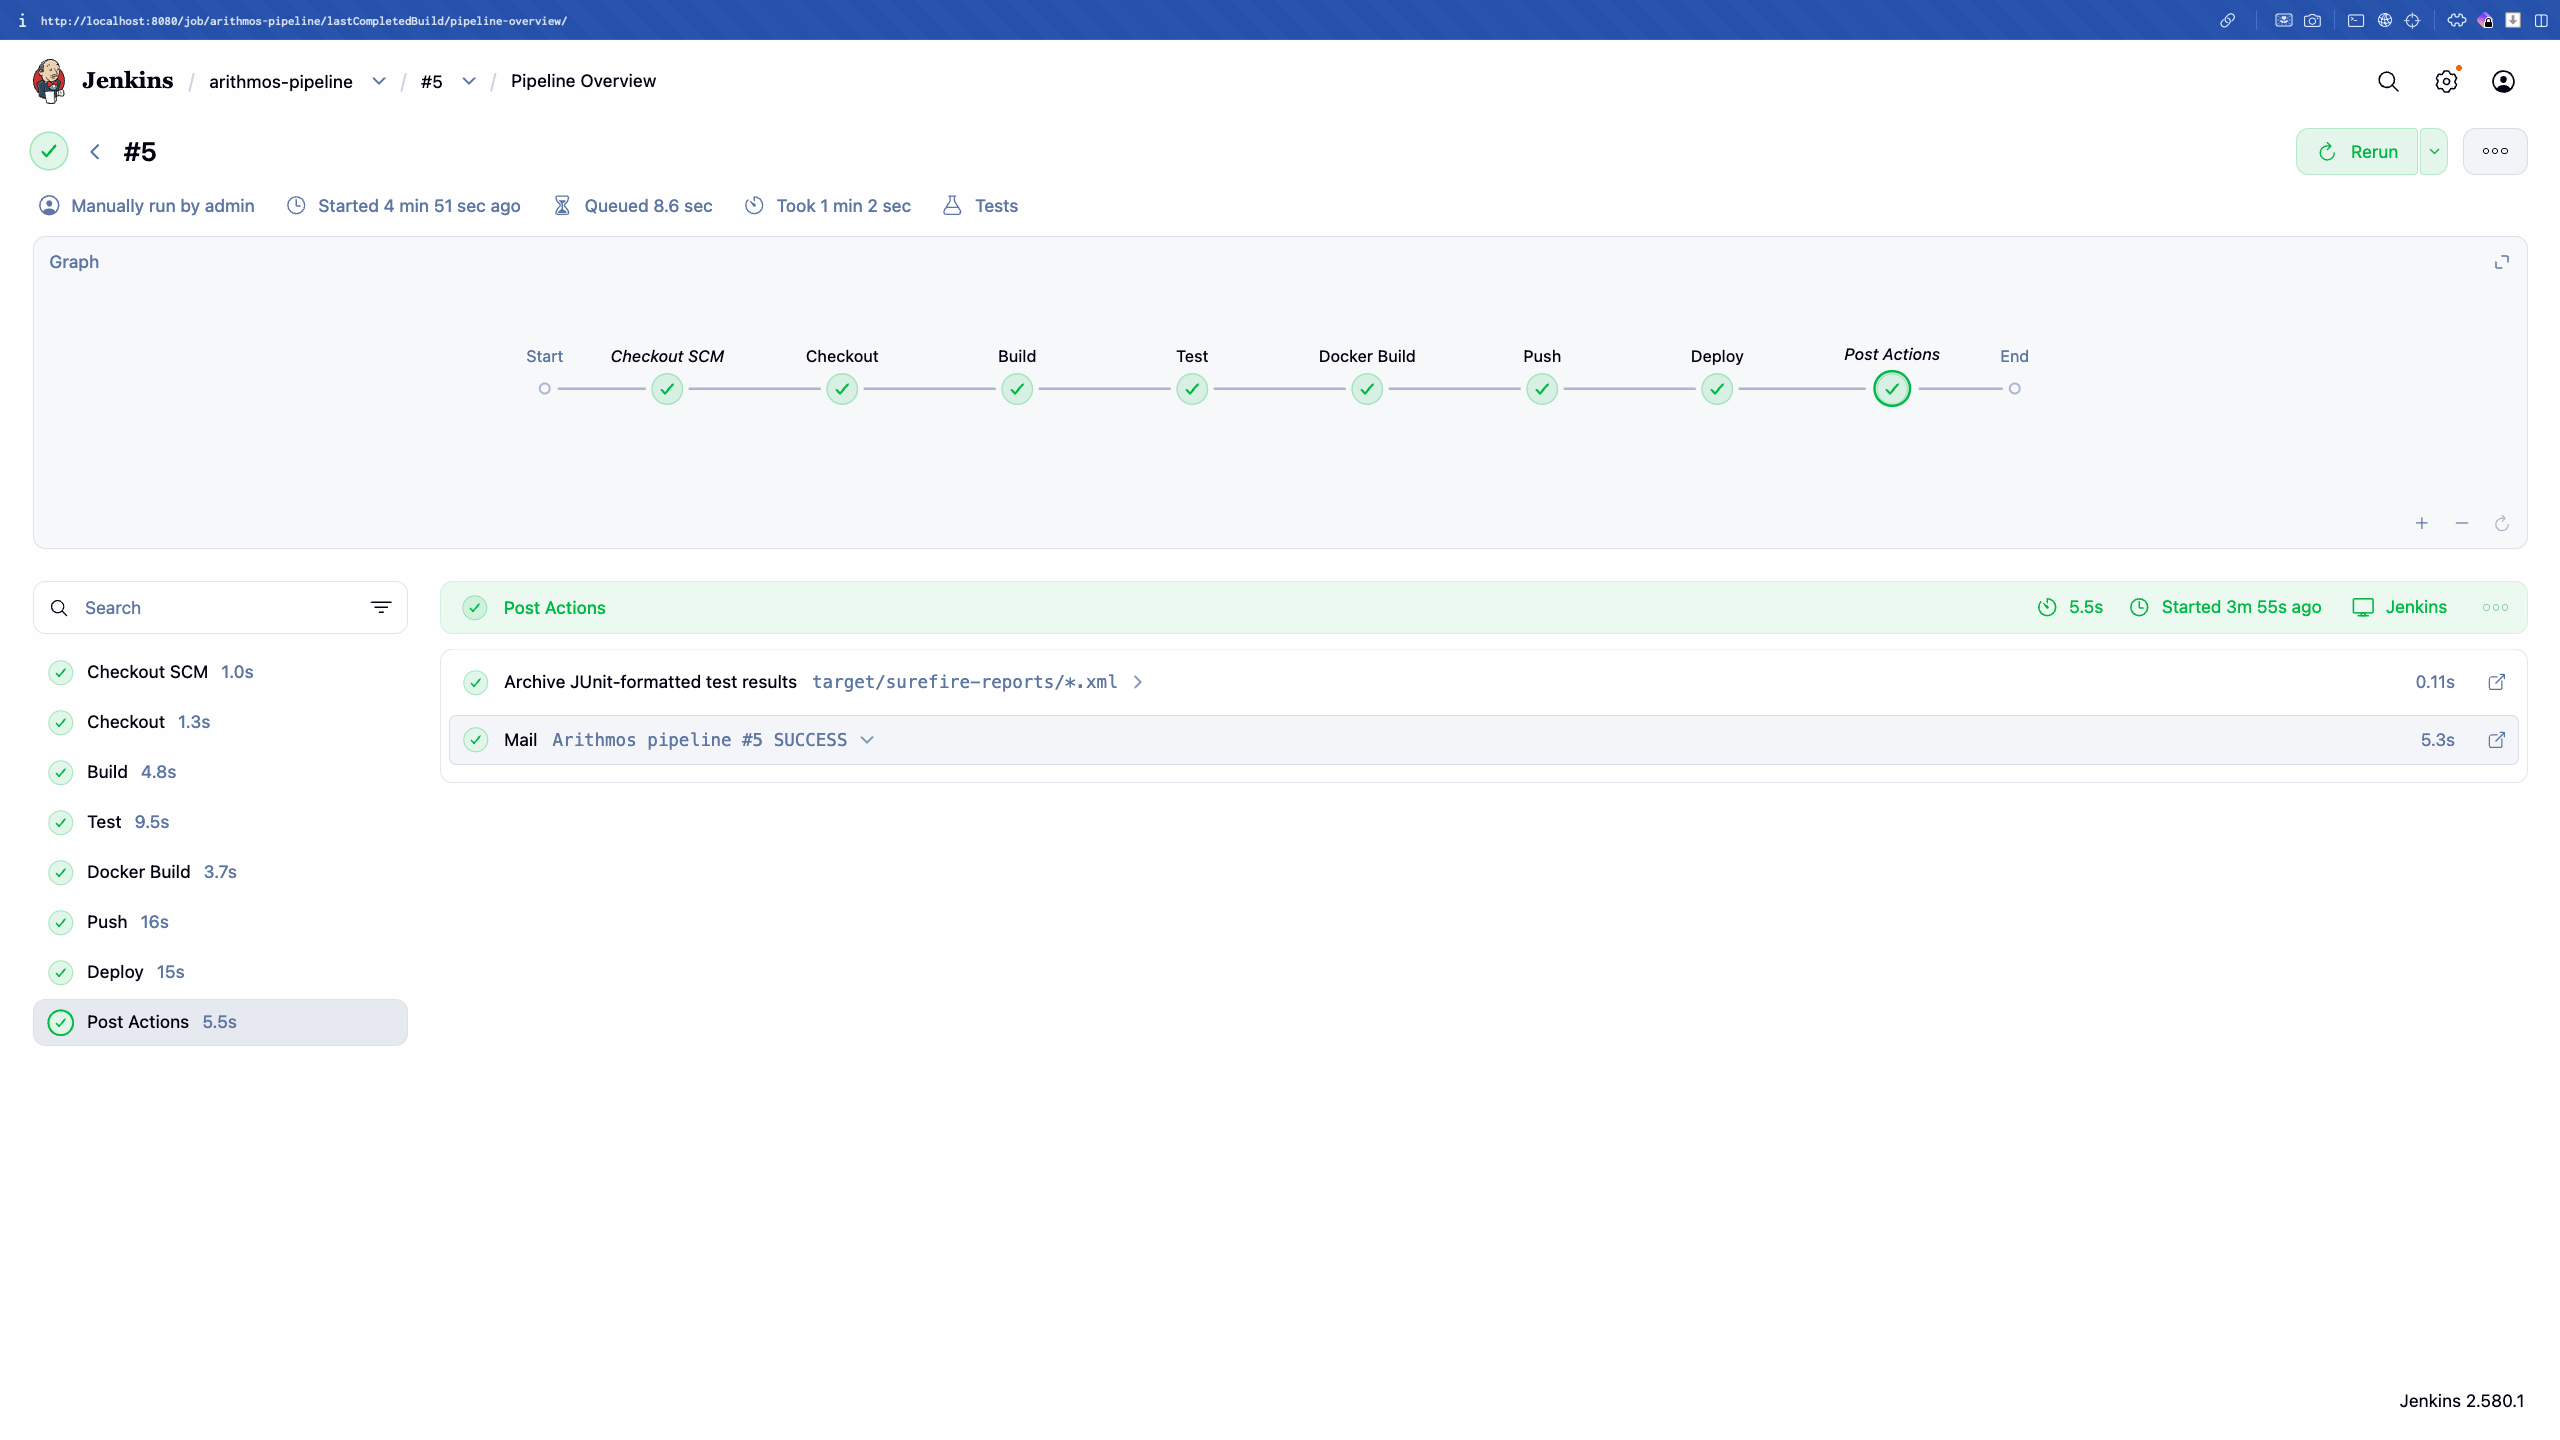
\includegraphics[width=\linewidth]{../screenshots/jenkins_job.png}\\
{\small Green pipeline run (build~\#5): all stages and post actions green.}
\\[6pt]
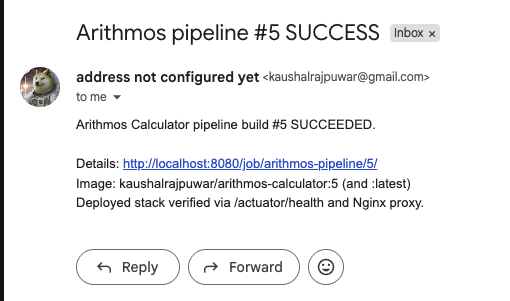
\includegraphics[width=0.62\linewidth]{../screenshots/email_confirmation.png}\\
{\small Build status email notification.}
\\[6pt]
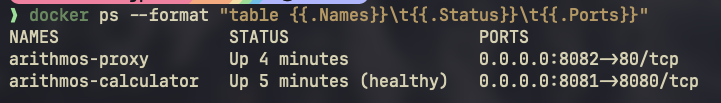
\includegraphics[width=0.85\linewidth]{../screenshots/docker_ps.png}\\
{\small \texttt{docker ps}: both containers up, calculator healthy.}
\\[6pt]
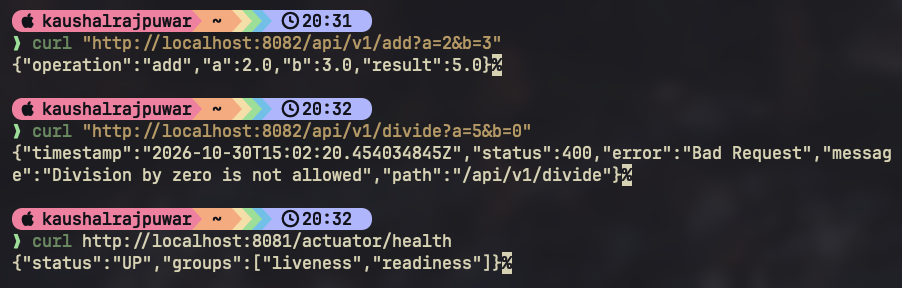
\includegraphics[width=0.9\linewidth]{../screenshots/api_responses.png}\\
{\small Live API: add via proxy, divide-by-zero 400, actuator health.}
\end{center}

\section{Challenges faced}
\textbf{Java version skew:} Jenkins' default \texttt{PATH} resolved
Java~27 while the project targets 21, and Mockito's inline mock maker
cannot run on 27 --- all MockMvc tests errored. Fixed by pinning
\texttt{JAVA\_HOME}/\texttt{PATH} to the Homebrew Java~21 install in the
\texttt{Jenkinsfile} environment block. \textbf{Deploy conflicts:}
leftover containers from manual testing collided with Jenkins'
\texttt{compose up} (same container names, different Compose project
directories). Fixed by making Deploy idempotent with
\texttt{down --remove-orphans} first. \textbf{Email:} no SMTP server
listened on \texttt{localhost:25}; configured the Jenkins mailer for
Gmail SMTP (port~587, app password held in the Jenkins credentials
store, never committed) and verified delivery. \textbf{Webhook:}
GitHub rejects \texttt{localhost} webhook URLs, and no tunnel tool was
available, so GitHub-to-Jenkins push delivery relies on the spec-allowed
Poll SCM fallback while \texttt{githubPush()} stays configured for a
public Jenkins URL. No credentials or secrets were ever committed; the
repository history (feature branch + pull request + progressive fixes)
is intentionally granular.

\end{document}
